%%%%%%%%%%%%%%%%%%%%%%%%%%%%%%%%%%%%%%%%%%%%%%%%%%%%%%%%%%%%%%%%
%% This file is the Main-File of the TexReportsTemplate       %%
%%               (c) by Tristan Wehrmaker                     %%
%%              last modified:  09/03/2021 (Anna Malinovskaya)%%
%%%%%%%%%%%%%%%%%%%%%%%%%%%%%%%%%%%%%%%%%%%%%%%%%%%%%%%%%%%%%%%%

\documentclass[11pt]{scrreprt}

%Pakete laden
%%%%%%%%%%%%%%%%%%%%%%%%%%%%%%%%%%%%%%%%%%%%%%%%%%%
%% This file is a part of the TexReportsTemplate %%
%%           (c) by Tristan Wehrmaker            %%
%%          last modified:  04/15/2008           %%
%%%%%%%%%%%%%%%%%%%%%%%%%%%%%%%%%%%%%%%%%%%%%%%%%%%

%Pakete für Seitenformat
\usepackage{geometry}
%\usepackage{showframe}
\usepackage{printlen}
\usepackage[automark]{scrpage2}
\usepackage{titlesec}
\usepackage{lscape}

%Pakete für Schriften
\usepackage[utf8]{inputenc}
%\usepackage[T1]{fontenc}
\usepackage{dsfont}
\usepackage{paralist}
%\usepackage{marvosym}
\usepackage{booktabs}
\newcommand {\otoprule }{\midrule[\heavyrulewidth]}
\newcommand{\ra}[1]{\renewcommand{\arraystretch}{#1}}

%Pakete für deutsche Sprache
%\usepackage{ngerman}
%\usepackage{ae}
\usepackage[english]{babel}

%Pakete für Farben
\usepackage{color}
\usepackage{colortbl}
\usepackage{xcolor}

%Pakete für Listings
\usepackage{listings}

%Pakete für Grafiken
\ifpdfoutput{\usepackage[pdftex]{graphicx}}{\usepackage{graphicx}}

%Mathematik-Pakete
\usepackage{amssymb}
\usepackage{amsmath}
\usepackage{amsthm}
\usepackage{cancel}

%Anklickbares Verzeichnis für PDF
\usepackage{hyperref}

%Serifenlose Schrift
%\usepackage[standard-baselineskips]{cmbright}

%Akronyme
\usepackage{acronym}

%Pakete für die Bibliographie
%\usepackage{bibgerm}
\usepackage{url}
\usepackage{float}
\usepackage{floatflt}
\usepackage{array}
\usepackage{fancybox}
\usepackage{framed}
%\usepackage{subfigure}
\usepackage{wasysym}
\usepackage{pifont}
\usepackage{algorithm}
\usepackage[noend]{algpseudocode}
\usepackage{mathtools}
\DeclarePairedDelimiter\ceil{\lceil}{\rceil}
\DeclarePairedDelimiter\floor{\lfloor}{\rfloor}

% comp packages
\usepackage{graphicx}
\usepackage{subfig}
\usepackage{caption}
\usepackage{lscape} 

% todo environment
\usepackage[show]{chato-notes}
\usepackage{comment}

%Paragraph margin
\usepackage[parfill]{parskip}


\newcommand{\specialcell}[2][c]{%
  \begin{tabular}[#1]{@{}l@{}}#2\end{tabular}}
  
\usepackage{mathtools}
\usepackage{flexisym} % textprime

%spacing tab
\newcommand{\itab}[1]{\hspace{0em}\rlap{#1}}
\newcommand{\tab}[1]{\hspace{.2\textwidth}\rlap{#1}}

\usepackage{hyperref}
\usepackage{tablefootnote}

%\usepackage[toc,page]{appendix}
\usepackage[]{appendix}

\usepackage{threeparttable}

\usepackage{cite}

\interfootnotelinepenalty=10000

\usepackage[all]{nowidow}

\renewcommand*{\chapterheadstartvskip}{\vspace*{0cm}}
\renewcommand*{\chapterheadendvskip}{\vspace*{2\baselineskip}}

\RedeclareSectionCommands[
beforeskip=-.5\baselineskip,
afterskip=.25\baselineskip
]{section,subsection,subsubsection}
\RedeclareSectionCommands[
beforeskip=.5\baselineskip,
afterskip=-1em]{paragraph,subparagraph}


%Variablen definieren
%%%%%%%%%%%%%%%%%%%%%%%%%%%%%%%%%%%%%%%%%%%%%%%%%%%
%% This file is a part of the TexReportsTemplate %%
%%           (c) by Tristan Wehrmaker            %%
%%          last modified:  04/15/2008           %%
%%%%%%%%%%%%%%%%%%%%%%%%%%%%%%%%%%%%%%%%%%%%%%%%%%%

\newcommand{\documentdate}{\today}

\newcommand{\documenttitle}{
Statistical Monitoring of Image Data %\\
}
% TODO: fix
\newcommand{\documentsubject}{Institut für Kommunikationstechnik}
\newcommand{\documentkeywords}{CVAE ect.}
\newcommand{\documentauthor}{Xilin Huang}
\newcommand{\documentlocation}{Hannover}
\newcommand{\documenttype}{Studienarbeit}
\newcommand{\documentcourse}{Mechatronik und Robotik}
\newcommand{\documentinstitute}{
Gottfried Wilhelm Leibniz Universität\\ 
Hannover, Germany\\
\vspace{2\baselineskip}
}
\newcommand{\documenttutor}{
\textbf{Mentor: M. Sc. }\\
\textbf{Examiner: Prof. Dr.}\\
\textbf{Examiner: Prof. Dr.}\\
}

%Konfiguration laden
%%%%%%%%%%%%%%%%%%%%%%%%%%%%%%%%%%%%%%%%%%%%%%%%%%%
%% This file is a part of the TexReportsTemplate %%
%%           (c) by Tristan Wehrmaker            %%
%%          last modified:  04/15/2008           %%
%%%%%%%%%%%%%%%%%%%%%%%%%%%%%%%%%%%%%%%%%%%%%%%%%%%

%Einstellungen für Seitenformat
\geometry{a4paper}
\uselengthunit{cm}
\topmargin-1.5cm
\headheight1cm
%\headsep0.1cm
\headsep0.8cm
\addtolength{\textheight}{3.4cm}
\topskip0.8cm
\textwidth15.0cm
\oddsidemargin0.5cm
\evensidemargin0.6cm

% nothing set
% textwidth: 418.25368pt, 14.69785 cm
% evensidemargin: 17.3571pt, 0.60994 cm
% oddsidemargin: 17.3571pt, 0.60994 cm
% topmargin: -8.26335pt, -0.29037 cm
% headheight: 0.5974 cm
% headsep: 0.71687 cm
% textheight: 20.78696 cm
% topskip: 0.38655 cm


\renewcommand{\baselinestretch}{1.2}
%\parindent0mm % either normal parindent or no parinden + parskip!

%Einstellungen für Farben
\definecolor{lightgray}{rgb}{0.7, 0.7, 0.7}
\definecolor{lightergray}{rgb}{0.85, 0.85, 0.85}
\definecolor{lightred}{rgb}{1.0, 0.5, 0.5}

%Einstellungen für Listings
\lstset{%
	basicstyle=\small\normalfont\tt\hyphenchar\font\m@ne\@noligs,
	frame=single,
	captionpos=b,
	lineskip=-1pt,
	basewidth=0.5em,
	breaklines,
	aboveskip=20pt,
	belowskip=\medskipamount%
}

%Anklickbares Verzeichnis für PDF
\hypersetup{%
   pdftitle={\documenttitle},
   pdfsubject={\documentsubject},
   pdfkeywords={\documentkeywords},
   pdfauthor={\documentauthor},
   colorlinks=true,
   linkcolor=black,
   citecolor=black,
   bookmarksopen=true,
   urlcolor=black,
   %Test
   plainpages=false,
   pdfpagelabels,
   hypertexnames=false}


%Serifenbehaftete Schrift für Überschriften
\setkomafont{sectioning}{\normalfont\normalcolor\bfseries}

%nach Paragraph neue Zeile anfangen
\titleformat{\paragraph}[hang]{\normalfont\bfseries}{}{0pt}{}

%Befehle zur Verfügung stellen
%%%%%%%%%%%%%%%%%%%%%%%%%%%%%%%%%%%%%%%%%%%%%%%%%%%
%% This file is a part of the TexReportsTemplate %%
%%           (c) by Tristan Wehrmaker            %%
%%          last modified:  04/15/2008           %%
%%%%%%%%%%%%%%%%%%%%%%%%%%%%%%%%%%%%%%%%%%%%%%%%%%%

% \newcommand{\comment}[1]{
% 	~\vspace{0.2cm}\\
% 	\fbox{
% 	\begin{minipage}[t]{13cm}
% 	      \textcolor{red}{\textbf{#1}}
% 	\end{minipage}
% 	}
% 	~\vspace{0.2cm}\\
% }

\newcommand{\items}[1]{
	~\vspace{0.2cm}\\
	\framebox[\textwidth]{
		\begin{tabular}{m{1.2cm}m{14cm}}
			\includegraphics[height=1cm]{Pics/gp.jpg} &
			\begin{itemize}#1\end{itemize}
		\end{tabular}
	}
	~\vspace{0.2cm}\\
}

\newcommand{\missing}{ \colorbox{red}{\textbf{...}} }

\newcommand{\recheck}[1]{ \colorbox{green}{\textbf{#1}} }

\newcommand{\multicomment}[1]{{}}

\newcommand{\marker}[1]{\textcolor{red}{#1}}

%\newcommand{\image}[2]{
%	\begin{figure}[h]
%		\begin{center}
%			\includegraphics{Pics/#1}
%			\caption{#2}
%		\end{center}
%	\end{figure}
%}
%\newcommand{\ok}{\includegraphics{Pics/check.png}}
\newcommand{\ok}{\ding{52}}

\newcommand{\image}[2]{
	\begin{figure}[h]
		\begin{center}
			\includegraphics{Pics/#1}
			\vspace{-0.2cm}
			\caption{#2}
		\end{center}
	\end{figure}
}

\newcommand{\imagewithtext}[3]{
	\begin{figure}[h]
		\begin{center}
			\includegraphics{Pics/#1}
			\caption{#2}
			~\\
			#3
		\end{center}
	\end{figure}
}

\newcommand{\fullsizeimage}[2]{
	\begin{figure}[h]
		\begin{center}
			\includegraphics[width=\textwidth]{Pics/#1}
			\caption{#2}
		\end{center}
	\end{figure}
}

%\newcommand{\qed}{\begin{flushright}q.e.d.\end{flushright}}
%\newcommand{\Rm}{\ensuremath{\mathds{R}}}
%\newcommand{\Rn}{\ensuremath{\mathds{N}}}
%\newcommand{\Rq}{\ensuremath{\mathds{Q}}}
%\newcommand{\Rc}{\ensuremath{\mathds{C}}}
%\newcommand{\Rz}{\ensuremath{\mathds{Z}}}
%\newcommand{\Reins}{\ensuremath{\mathds{1}}}
%\newcommand{\Pot}{\operatorname{Pot}}
%\newcommand\pmat[1]{\begin{pmatrix} #1\end{pmatrix}}
%\newcommand{\Kdots}{,\ldots,}
%\newcommand{\Dotdots}{\cdot \ldots \cdot}
%\newcommand{\Midots}{- \ldots -}
%\newcommand{\Pludots}{+ \ldots +}
%\newcommand{\Indi}{{1\hspace{-1.7mm}\bot}}
%-----------------------------Suetterlin---------------------------------------
%\newcommand{\SA}{\text{{\suet A} }}
%\newcommand{\SP}{\text{{\suet P} }}
%\newcommand{\SL}{\text{{\suet L} }}

%-----------------------------Math-Operators----------------------------------
\DeclareMathOperator{\id}{id}
\DeclareMathOperator{\K}{Kern}
\DeclareMathOperator{\rang}{rang}
\DeclareMathOperator{\sh}{Sh}
\DeclareMathOperator{\spgl}{S_L}
\DeclareMathOperator{\arctanh}{arctanh}
\DeclareMathOperator{\arcoth}{arcoth}
\DeclareMathOperator{\Basis}{Basis}
\DeclareMathOperator{\Bild}{Bild}

\newcommand{\work}{
\label{Workpoint}
\fcolorbox{black}{lightred}{\textbf{W}}
}

\newtheoremstyle{mydef}	% name
	{10pt}				% Space above 
	{10pt}				% Space below 
	{\itshape}			% Body font 
	{}					% Indent amount 1
	{\bfseries}			% Theorem head font 
	{:}					% Punctuation after theorem head 
	{.5em}				% Space after theorem head 2
	{}					% Theorem head spec (can be left empty, meaning `normal')
						%1 Indent amount: empty = no indent, \parindent = normal paragraph indent
						%2 Space after theorem head: { } = normal interword space; \newline = linebreak

\theoremstyle{mydef}
\newtheorem{Def}{Definition}

%Workaround für \lstlistoflistings
\makeatletter
\@ifundefined{float@listhead}{}{%
    \renewcommand*{\lstlistoflistings}{%
        \begingroup
    	    \if@twocolumn
                \@restonecoltrue\onecolumn
            \else
                \@restonecolfalse
            \fi
            \float@listhead{\lstlistlistingname}%
            \setlength{\parskip}{\z@}%
            \setlength{\parindent}{\z@}%
            \setlength{\parfillskip}{\z@ \@plus 1fil}%
            \@starttoc{lol}%
            \if@restonecol\twocolumn\fi
        \endgroup
    }%
}
\makeatother

\newenvironment{tabularcompactitem}{%
  \setdefaultleftmargin{1em}{1em}{1em}{1em}{1em}{1em}%
  \vspace{-\topsep}%
  \compactitem
}{
  \vspace*{-\ht\strutbox}%
  \endcompactitem
}

\let\oldtabular=\tabular
\def\tabular{\small\oldtabular}

%\let\oldlstlisting=\lstlisting
%\def\lstlisting{\vspace{-0.5cm}\oldlstlisting}

\definecolor{lightgray}{gray}{0.8}
\definecolor{lightblue}{rgb}{0.51,0.68,0.91}

%Titelseite definieren
%%%%%%%%%%%%%%%%%%%%%%%%%%%%%%%%%%%%%%%%%%%%%%%%%%%
%% This file is a part of the TexReportsTemplate %%
%%           (c) by Tristan Wehrmaker            %%
%%          last modified:  04/15/2008           %%
%%%%%%%%%%%%%%%%%%%%%%%%%%%%%%%%%%%%%%%%%%%%%%%%%%%




\title{
    \vspace{-1cm}
    
\includegraphics[scale=0.8]{images/leibniz.png}\\
	\vspace{1cm}
	\Large{\documentinstitute}
	\vspace{1cm}
	\Large{\documenttype}
	\vspace{0.4cm}\\
	\huge{\textbf{\documenttitle}}
	\vspace{1.0cm}\\
	%\vspace{2cm}\\
	%\Large{\documenttype}
	%\vspace{1cm}\\
	%\textnormal{in \documentcourse}
	%\vspace{0.6cm}\\
	%\textnormal{by}
	\Large\textbf{\documentauthor}
	\vspace{1cm}\\
	\documenttutor
	\vspace{2cm}
	
\includegraphics[scale=0.8]{images/IKT.png}\hspace{1cm}
	
\includegraphics[scale=0.6]{images/IKG.png}\\
	\vspace{-1cm}
}





%Dokument beginnen
\begin{document}


%Kopf- und Fusszeilen definieren
\clearscrheadfoot
\ihead{\textbf{\headmark}\hfill }

\setheadsepline{.9pt}   % Linie zwischen Kopf und Text
%\setfootsepline{.9pt}   % Linie zwischen Text und Fuß

\renewcommand*{\chapterpagestyle}{scrheadings}
\pagestyle{scrheadings}

\cfoot{\textbf{\pagemark}}

% \noindent
% textwidth: \the\textwidth, \printlength{\textwidth}\\
% evensidemargin: \the\evensidemargin, \printlength{\evensidemargin}\\ 
% oddsidemargin: \the\oddsidemargin, \printlength{\oddsidemargin}\\
% topmargin: \the\topmargin, \printlength{\topmargin}\\
% headheight: \printlength{\headheight}\\
% headsep: \printlength{\headsep}\\
% textheight: \printlength{\textheight}\\
% topskip: \printlength{\topskip}\\

%15 cm textwidth, no margins set
%textwidth: 426.79134pt, 14.99786 cm
%evensidemargin: 17.3571pt, 0.60994 cm
%oddsidemargin: 17.3571pt, 0.60994 cm
%topmargin: -42.67912pt, -1.49979 cm

% nothing set
% textwidth: 418.25368pt, 14.69785 cm
% evensidemargin: 17.3571pt, 0.60994 cm
% oddsidemargin: 17.3571pt, 0.60994 cm
% topmargin: -8.26335pt, -0.29037 cm
% headheight: 0.5974 cm
% headsep: 0.71687 cm
% textheight: 20.78696 cm
% topskip: 0.38655 cm




%Titelseite erstellen
\maketitle

%master thesis protocol
\thispagestyle{empty}
\underline{\large{\textbf{protocol of statistical monitoring of image data}}}

\vspace{1cm}
The purpose of this research is to propose a feasible method to monitor the change image data with the help of statistical method and control chart. 

The goal of this thesis is to find out a statik to accuratlly represent to state of image data.



\section*{Methodology}
\textit{Algorithm:} statistical based defect detection, e.g., maximun variance of sliding windows, Discrete wavelet transform. \\
\textit{Framework:} control chart e.g., Shewhart control chart, $\chi^{2}$ control chart, Hotelling $T^{2}$ control chart.   \\
%\textit{Datasets:}   \\
\textit{Programming language:} Matlab.


\section*{Tasks with Tentative Schedule}
\begin{itemize}
    \item The first and the second months: literature review and data collect
    \item The second to the forth months: empirical study and hypotheses propose
    \item The forth and the fifth month: test and modify the proposed hypotheses
    \item The sixth month: writing and presenting thesis
    \item The end: evaluation of performance (including thesis and presentation)
\end{itemize}



%Erklärung hinzufügen
\newpage
%%%%%%%%%%%%%%%%%%%%%%%%%%%%%%%%%%%%%%%%%%%%%%%%%%%
%% This file is a part of the TexReportsTemplate %%
%%           (c) by Tristan Wehrmaker            %%
%%          last modified:  04/15/2008           %%
%%%%%%%%%%%%%%%%%%%%%%%%%%%%%%%%%%%%%%%%%%%%%%%%%%%

\thispagestyle{empty}
	\begin{abstract}
	\begin{center}
		%\Large{\textbf{Erklärung}}\\
	\huge{\textbf{Statutory Declaration}}\\
	\vspace{2cm}
    \large{I, \textcolor{red}{YOUR NAME}, declare that this master's thesis, and the work indicated herein have been composed by myself, and any sources have not been used other than those specified. All the consulted published or unpublished work of others have been clearly cited. I additionally declare that the work and master's thesis have not been submitted for any other previous degree examinations.}\\
	\end{center}
	~\\
	%Hiermit versichere ich, dass ich die vorliegende \documenttype{} selbstständig und ohne fremde Hilfe
	%verfasst und keine anderen als die in der Arbeit angegebenen Quellen und Hilfsmittel verwendet
%habe.

	\rule{\textwidth}{0.5pt}
	\documentauthor\hfill \documentlocation, \documentdate
    \begin{center}
		%\Large{\textbf{Erklärung}}\\
		
	\vspace{3cm}
	\huge{\textbf{Eidesstattliche Erklärung}}\\
	\vspace{2cm}
    \large{Ich, \textcolor{red}{YOUR NAME}, erkläre hiermit, die Arbeit selbstständig verfasst zu haben und keine anderen als die angegebenen Quellen und Hilfsmittel benutzt zu haben. Alle Stellen der Arbeit, die wörtlich oder sinngemäß aus anderen Quellen übernommen wurden, habe ich als solche kenntlich gemacht. Die Arbeit wurde in gleicher oder ähnlicher Form noch keiner Prüfungsbehörde vorgelegt.}\\
	\end{center}
    ~\\
    \rule{\textwidth}{0.5pt}
    \\
    \documentauthor\hfill \documentlocation, \documentdate
\end{abstract}


%acknowledgements
%%%%%%%%%%%%%%%%%%%%%%%%%%%%%%%%%%%%%%%%%%%%%%%%%%%
%% This file is a part of the TexReportsTemplate %%
%%           (c) by Tristan Wehrmaker            %%
%%          last modified:  04/15/2008           %%
%%%%%%%%%%%%%%%%%%%%%%%%%%%%%%%%%%%%%%%%%%%%%%%%%%%

\thispagestyle{empty}
	\begin{abstract}
		\begin{center}
			\textbf{Acknowledgements}\\
			~\\
			\textit{
			    Throughout the writing of this thesis, I have received a great deal of support and assistance. I would first like to thank Du Qinyang from BYD company for providing mobile phone cover images used in experiments. In addition, I would first like to thank my supervisor, Anna Malinovskaya, whose expertise was invaluable in formulating the research questions and methodology. Your insightful feedback pushed me to sharpen my thinking and brought my work to a higher level.
				}
			
		\end{center}
	\end{abstract}
\newpage


%Zusammenfassungen einfügen
%%%%%%%%%%%%%%%%%%%%%%%%%%%%%%%%%%%%%%%%%%%%%%%%%%%
%% This file is a part of the TexReportsTemplate %%
%%           (c) by Tristan Wehrmaker            %%
%%          last modified:  04/15/2008           %%
%%%%%%%%%%%%%%%%%%%%%%%%%%%%%%%%%%%%%%%%%%%%%%%%%%%

%Abstract
%\thispagestyle{empty}


\begin{abstract}
\begin{center}
%\vspace{-1cm}
\textit{Abstract}
\end{center}

%\vspace{\baselineskip}
%\begin{minipage}{12cm}
%\parskip = 12pt
Here write your abstract for your thesis. Please keep it accurate and clear within one page.

%\end{minipage}

\end{abstract}

\newpage

%Danksagung einfügen
%%%%%%%%%%%%%%%%%%%%%%%%%%%%%%%%%%%%%%%%%%%%%%%%%%%%
%% This file is a part of the TexReportsTemplate %%
%%           (c) by Tristan Wehrmaker            %%
%%          last modified:  04/15/2008           %%
%%%%%%%%%%%%%%%%%%%%%%%%%%%%%%%%%%%%%%%%%%%%%%%%%%%

\thispagestyle{empty}
	\begin{abstract}
		\begin{center}
			\textbf{Acknowledgements}\\
			~\\
			\textit{
			    Throughout the writing of this thesis, I have received a great deal of support and assistance. I would first like to thank Du Qinyang from BYD company for providing mobile phone cover images used in experiments. In addition, I would first like to thank my supervisor, Anna Malinovskaya, whose expertise was invaluable in formulating the research questions and methodology. Your insightful feedback pushed me to sharpen my thinking and brought my work to a higher level.
				}
			
		\end{center}
	\end{abstract}
\newpage

%Inhaltsverzeichnis erstellen
\tableofcontents

%Akronyme hinzufügen
%%%%%%%%%%%%%%%%%%%%%%%%%%%%%%%%%%%%%%%%%%%%%%%%%%%%
%% This file is a part of the TexReportsTemplate %%
%%           (c) by Tristan Wehrmaker            %%
%%          last modified:  04/15/2008           %%
%%%%%%%%%%%%%%%%%%%%%%%%%%%%%%%%%%%%%%%%%%%%%%%%%%%

%List of Acronyms
\chapter*{List of Acronyms}

\begin{acronym}[XHTML]
%Here you need to list all the acronyms that appear in your thesis main content. For example:

    \vspace{2cm}
    \acro{AI}{Artificial Intelligence}
    \acro{CNNs}{Conventional Neural Networks}
    \acro{DL}{Deep Learning}
    \acro{FNNs}{Feedforward Neural Networks}
    \acro{GPU}{Graphics Processing Unit}
    \acro{GRUs}{Gated Recurrent Units}
    \acro{IDE}{Integrated Development Environment}
    \acro{KLD}{Kullback-Leibler divergence}
    \acro{LIDAR}{Light Detection and Ranging}
    \acro{LSTM}{Long Short-Term Memory}
    \acro{ML}{Machine Learning}
    \acro{NLP}{Natural Language Processing}
    \acro{RNNs}{Recurrent Neural Networks}
    \acro{SGD}{Stochastic Gradient Descent}
    \acro{SDD}{Stanford Drone Dataset}

    
    
    
    
    

    
    


\end{acronym}


%----------------------------- INHALT -----------------------------

%Abbildungsverzeichnis hinzufügen
\listoffigures

\clearpage
%Tabellenverzeichnis hinzufügen
%\begin{minipage}{\textwidth}
%\listoftables
%\end{minipage}

%Kapitel hinzufügen
%%%%%%%%%%%%%%%%%%%%%%%%%%%%%%%%%%%%%%%%%%%%%%%%%%%
%% This file is a part of the TexReportsTemplate %%
%%           (c) by Tristan Wehrmaker            %%
%%          last modified:  04/15/2008           %%
%%%%%%%%%%%%%%%%%%%%%%%%%%%%%%%%%%%%%%%%%%%%%%%%%%%
% introduction
\chapter{Introduction}
\label{cp:Introduction}

Here is the introduction. You need to write the following key points for your work. Keep each part concise and short. In total, this chapter should not be more than four pages.

The remainder of this paper is organized as follows. The
real-time contrasts framework for image monitoring is
introduced in Section 2. Section 3 evaluates the performance
of the proposed method using simulations. Section 4
provides an experiment to apply the proposed method in an
industrial environment. Finally, the conclusions and
directions of future research are presented.

\begin{itemize}
    \item Background
    \item Motivation
    \item Research gap
    \item Objectives
    \item Approach (in introduction chapter you do not necessarily need to write the results for your work)
    \item The structure of your thesis
\end{itemize}
\chapter{Related Work}
\label{cp:RelatedWork}


Here you need to write your related work and cite properly. For example, one of the most influential researchers in ~\ac{DL} is Yann LeCun with the Nature Article \textit{Deep learning} \cite{lecun2015deep}. In total, you should refer to preferably approximately 50 papers (not less than 40 papers).

Here, it is highly recommended to start writing this part as soon as you start reading any papers. It will take you a lot of time to do so and can also help you track the papers that you have been reading.



 
\chapter{Background}
\label{cp:Background}

\begin{comment}
Please write down the basic background for your research, e.g., the fundamental concepts of the approaches that you use in the thesis, so that other people (who do not have the background) can understand your work.

Here is one example for sigmoid function:

The sigmoid function is defined by formula~\ref{eq:sigmoid}. It can compress the input into the interval $(0, 1)$. The drawback of the sigmoid activation function is the so-called ``kill gradients'': if the input values locate in the tail of 0 or 1, the gradient at these regions tend to be zero. If the sigmoid function is used multiple times in a neural network, the gradients may be very small or even disappear.

\begin{equation}
\label{eq:sigmoid}
\centering{f(x) = \frac{1}{1 + e^{-x}}}.
\end{equation}
\end{comment}

\section{Discrete wavelet decomposition}


\section{Hotteling $T^{2}$ control chart}

There are two distinct phases of the control chart
~\cite{bersimis2007multivariate}.

\begin{itemize}
\item Phase I: charts are used for retrospectively testing whether the process was in control when the first
subgroups were being drawn. In this phase, the charts are used as aids to the practitioner, in bringing a
process into a state where it is statistically in control.
\item Phase II: control charts are used for testing whether the process remains in control when future subgroups
are drawn. In this phase, the charts are used as aids to the practitioner in monitoring the process for any
change from an in-control state.
\end{itemize}






\chapter{Methodology}
\label{cp:Methodology}

  The proposed framework uses a bottom-up pipeline to
gradually infer a high-level representation of the scratches and stains from low-level features in a back cover of mobile phone image. Firstly by mean of the wavelet transform, the surface texture properties such as scratch and stain are decomposed into so-called wavelet characteristics. Then multivariate statistical approach, i.e. Hotelling $T^{2}$ control chart is utilized to monitor the mean vector of a multivariate process, which can be used to judge the existence of scratch defects in the sample image.

\section{Maximal variance of moving windows}
For the surface of the back cover of handy, we assume that the pixels of the back cover are homogeneous. Therefore, we thought of using the variance of the pixel value to extract some features to represent the surface state. 


The control charts are used spatially by moving a mask (or window) across the image and then calculating and plotting a statistic each time the mask is moved. The size of the mask depends on the expected size of the defects to be detected, with smaller defective regions requiring smaller mask sizes.~\cite{megahed2011review}Inspired by this view, we move a 10 by 10 window across the image and calculate the variance of the pixel value each time the window is moved. Then value with the largest variance in this image is taken as the desired statistic describing this image.

\section{Discrete Wavelet transform decomposition}
  The continuous wavelet transform was computed by changing the scale of the analysis window, shifting the window in time, multiplying by the signal, and integrating over all times. In the discrete case, filters of different cutoff frequencies are used to analyze the signal at different scales. The signal is passed through a series of high pass filters to analyze the high frequencies, and it is passed through a series of low pass filters to analyze the low frequencies.


%~\cite{polikarTHE WAVELET TUTORIALusing}
  The DWT [Fig.~\ref{fig:dwt}] analyzes the signal at different frequency bands with different resolutions by decomposing the signal into a coarse approximation and detail information, which are associated with low pass and highpass filters, respectively. In our case, we use Haar discrete wavelet transform as the basic function to perform signal decomposition, so that an original image is decomposed into four coefficients: one low-pass filtering coefficients (approximation coefficients) and three high-pass filtering coefficients (detail coefficients, containing the horizontal(h), vertical(v), and diagonal(d) detail coefficients) at each level.

%Here is one example demonstrated by Fig.~\ref{fig:dwt} that adapted from~\cite{hijazi2015using}. 

\begin{figure}[h]
\centering
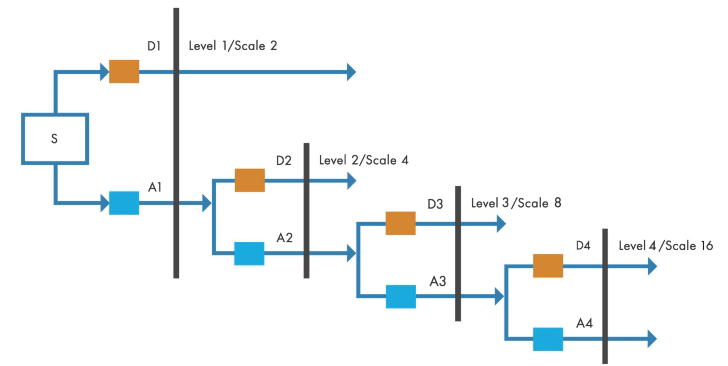
\includegraphics[width=1\textwidth]{images/dwt.png}
\caption[Structure of CNNs]{A general structure of CWT, the orange cube represent high-pass filter, the blue cube represent low-pass filter. Figure is adapted from MATLAB Tech Talks.}
\label{fig:dwt}
\end{figure}

  The number of coefficients of approximation coefficients and detail coefficients are halved when the level increase,since the images we analysized is in form of 2-D, so we need to perform the 2-D haar wavelet tranform by applying 1-D wavelet transform first on rows and then on columns.There is a built-in function in MATLAB haart2, which perform 2-D haar wavelet tranform.
the haart2 transform is obtained down to level

\begin{equation}
\log_2(min(row's dimension,column's dimension)) \label{equa:log1}
\end{equation}

 %\[\log_2(min(row's dimension,column's dimension))\] \label{equa:log1}
If the row or column dimension of data is even, but not a power of two, the haart2 transform is obtained down to level 

\begin{equation}
\lfloor \log_2(\frac{min(row's dimension,column's dimension)}{2}) \rfloor \label{equa:log2}
\end{equation}
%\[\lfloor \log_2(\frac{min(row's dimension,column's dimension)}{2}) \rfloor\] \label{equa:log2}

In our case, we have sample data of size 100 * 100, the largest level of haart2 transform is then 5 by using Equation \ref{equa:log2}.By using wavelet decomposition






\section{Wavelet decomposition based Hotteling $T^{2}$ control chart}
  In order to monitor the surface quality of the mobile phone, we need some feature quantities to characterize the quality of the image. The DWT are used to retrieved quality characteristics from image data, since It decomposes the image data into some details coefficients, which contain horizontal, vertical, and diagonal coefficients. These coefficients can be used as the input of the control chart after processing, and the control chart can then judge whether the procedure is under control by monitoring the value of the coefficient.


  A RGB image has three frame: R,G and B frame, we apply haar wavelet transform on each frame at the same time, the coefficients of final level have actually final level times filtered by high pass filter, which mean the amplitude of coefficients contain the information of high frequency signal in original image, namely The higher the coefficients, the more likely the signal will be abrupt. The Abrupt in the signal then represent the defects in the products which we are monitoring.
% maybe I should try get 9 elements to represent a image, that's more reasonable


	After we decompose an image of ($M \times N$) pixels, we get horizontal(h), vertical(v), and diagonal(d) coefficient matrix($S \times S$) for each frame at final level($L$),each coefficient matrix have $S^2$ coefficients,an image sample can have $3 \times S^2$ coefficients.~\ref{montgomery2020introduction} present tables indicating the recommended number of quality characteristics p = 2, 3, 4, 5, 10, and 20. It turns out that the cooeficients of dianonal coefficient matrix can best reflects the surface defects of various shapes(see experiment ~\ref{cp:experiment}),thus we first absolute all coefficients, which turn negative coefficients into positive coefficients withoud changing the value of itself. After that we take the maximal coefficient among the diagonal matrix and consider it as the disired statistical charateristic of coresponding frame. Finally 3 coefficients retrieved from an image is composing the mean characteristic vector in Multivariate Control Chart. 


There are two distinct phases of the control chart~\cite{bersimis2007multivariate}.

\begin{itemize}
\item Phase I: charts are used for retrospectively testing whether the process was in control when the first
subgroups were being drawn. In this phase, the charts are used as aids to the practitioner, in bringing a
process into a state where it is statistically in control.
\item Phase II: control charts are used for testing whether the process remains in control when future subgroups
are drawn. In this phase, the charts are used as aids to the practitioner in monitoring the process for any
change from an in-control state.
\end{itemize}

Multivariate Control Chart can be utilized to simultaneous monitor more than one quality characteristic. 





\chapter{Dataset}
\label{cp:dataset}

Here you need to describe the dataset(s) that you use for your experiments. If you use some open--source data, please cite them properly.

Here is an example of the Stanford drone datasets (SDD)~\cite{robicquet2016learning}. \ac{SDD} provides a bird's-eye-view in various intersections on Stanford University campus. 

\begin{table}[h!]
\begin{centering}
\begin{tabular}{ | m{2cm} | m{2cm} | m{2cm} | m{2cm} | m{2cm} |} 
\hline
frame Nr. & user ID & x  & y  & user type \\ 
\hline
834 & 0 & 819.5 & 29.5 & 2 \\
\hline
835 & 0 & 819.5 & 29.5 & 2 \\
\hline
\end{tabular}
\caption[Real data of \ac{SDD}]{An example of the real data for \ac{SDD}~\cite{robicquet2016learning}. The first, second, third, fourth, and fifth column present the frame ID, user ID, x coordinates, y coordinates, and user type, respectively. The x and y coordinates are in pixels.} 
\label{table:real_data_sdd}
\end{centering}
\end{table}
\chapter{Experiments}
\label{cp:experiment}

Please wire the experiments you have been doing for your research problems in detail and in an understandable way. This is the part that will largely reflect the work you have been doing for your thesis and will also mainly decide whether you can pass the examination or not.

Please keep in mind that you backup your code properly and regularly to avoid any risks by accident. It is recommended to use some open--source platform such as GitHub\footnote{\url{https://github.com}}, which is also very convenient for code sharing.
\chapter{Summary and Outlook}
\label{cp:summary_outlook}

\section{Summary} \label{sec:summary}

\begin{comment}

Here you need to wrap up the thesis in very concise and short paragraph(s). This is normally a very frequent part that your readers take a first look. 

You can also change this sub-chapter to conclusion if you can draw a conclusion based on the results you have found. However, please pay attention to the difference between conclusion and summary.
\end{comment}


This study proposed a framework for applying SPC in the context of image data using feature extract techniques in the frequency domain to monitor mobile phone cover's surface quality. In this framework, two methods with different feature extract techniques and control charts are proposed and compared, namely wavelet transformation with Hotelling $T^{2}$ control chart, and maximum variance among sliding window in combination with Shewhart $\bar{X}$ control chart. After feature extraction with wavelet transformation and maximum variance, the detail coefficients are monitored over time using a Hotelling $T^{2}$ control chart and Shewhart $\bar{X}$ control chart, respectively. Average run length, $ASS$, and $FDR$, are considered in empirical studies to evaluate the performance of the proposed methods in detecting faults. The result turns out that the method with wavelet transformation with Hotelling $T^{2}$ control chart achieves better performance in detecting defects and is more robust under different testing conditions. A comparison experiment is conducted in samples with different colours with the same methods mentioned above. The result illustrates that method II have almost the same performance (in term of Average run length and $FDR$) as that in original image data, proving method II is more suitable in different test situations. 

\section{Outlook} \label{sec:outlook}

There are three limitations in method II of this study. First, the number of decomposed characteristics is too few in our case since we only use the maximum value among the $H$, $V$, and $D$ matrices as desire statistics, which did not take advantage of the information in $RGB$ frame. Whether more statistics retrieved from image data can achieve better performance needs further study. Although our proposed methods perform well in detecting defects, the detection results do not include the specific location of the defects, which is not conducive to the troubleshooting of the post-production process and the improvement of the process flow. Thus the determination of faults location is also an exciting yet valuable research direction. The final limitation is the efficient problem by mix colour samples sets. The feasibility of using the Phase I in-control parameters of a batch of samples as the Phase II input of another batch of samples deserves further study.


\chapter{Summary and Outlook}
\label{cp:summary_outlook}

\section{Summary} \label{sec:summary}
Here you need to wrap up the thesis in very concise and short paragraph(s). This is normally a very frequent part that your readers take a first look. 

You can also change this sub-chapter to conclusion if you can draw a conclusion based on the results you have found. However, please pay attention to the difference between conclusion and summary.

\section{Outlook} \label{sec:outlook}

Here you can point out some potential aspects or interesting directions for future work and improvement. 


%\newpage
%\appendix
%\input{Content/ChapterB-APIDoc.tex}


%--------------------------- INHALT ENDE --------------------------

%Bibliographie hinzufügen
\bibliography{bibliography}
\bibliographystyle{apalike}
%\bibliography{Content/0mycite}


%Listingverzeichnis hinzufügen
%\begin{minipage}{\textwidth}
%\lstlistoflistings
%\end{minipage}

\end{document}
